%
% Copyright © 2014 Sara Lelliott. All Rights Reserved.
%
\documentclass[letterpaper,12pt]{article}

%%%%%%%%%%%%%%%%%%%%%%%%%%%%%
%       LaTeX Packages      %
%%%%%%%%%%%%%%%%%%%%%%%%%%%%%
\usepackage[affil-it]{authblk}
\usepackage{wrapfig}
\usepackage{tikz}
\usetikzlibrary{mindmap}
\usepackage{hyperref}
\usepackage{verbatimbox}
%%%%%%%%%%%%%%%%%%%%%%%%%%%%%

%%%%%%%%%%%%%%%%%%%%%%%%%%%%%%%%%%%%%%
% Tweak title page for multi-authors %
%%%%%%%%%%%%%%%%%%%%%%%%%%%%%%%%%%%%%%
\makeatletter
\def\@maketitle{%
  \newpage
  \null
  \vskip 2em%
  \begin{center}%
  \let \footnote \thanks
    {\Large\bfseries \@title \par}%
    \vskip 1.5em%
    {\normalsize
      \lineskip .5em%
      \begin{tabular}[t]{c}%
        \@author
      \end{tabular}\par}%
    \vskip 1em%
    {\normalsize \@date}%
  \end{center}%
  \par
  \vskip 1.5em}
\makeatother
%%%%%%%%%%%%%%%%%%%%%%%%%%%%%%%%%%%%%%

%%%%%%%%%%%%%%%%%%
% Begin Document %
%%%%%%%%%%%%%%%%%%
\begin{document}
%.

%%%%%%%%%%%%%%%%%%%%%%%%%%%%% FIXME: emails..
% Primary document author %
\author{Sara Lelliott%
  \thanks{Electronic address: \href{mailto:slel0001@uni.sydney.edu.au}{unikey@uni.sydney.edu.au}; Corresponding author}}
\affil{Department of IT, University of Sydney}
% Co-authors %
\author{Claire Lloyd-Prior%
  \thanks{Electronic address: \href{mailto:unikey@uni.sydney.edu.au}{unikey@uni.sydney.edu.au}}}
\affil{Department of IT, University of Sydney}
\author{Robert Schroder%
  \thanks{Electronic address: \href{mailto:unikey@uni.sydney.edu.au}{unikey@uni.sydney.edu.au}}}
\affil{Department of IT, University of Sydney}
\author{Callum Swain%
  \thanks{Electronic address: \href{mailto:unikey@uni.sydney.edu.au}{unikey@uni.sydney.edu.au}}}
\affil{Department of IT, University of Sydney}
\author{Michal Wahnon%
  \thanks{Electronic address: \href{mailto:unikey@uni.sydney.edu.au}{unikey@uni.sydney.edu.au}}}
\affil{Department of IT, University of Sydney}
% Project Title %
\title{Website Project}
\date{Dated: \today}
%%%%%%%%%%%%%%%%%%%%%%%%%%%%%

%%%%%%%%%%%%%%%%%%%%%%%%%%%%%%%%%%%%%%%%%%%%%%%%%%%%%%%
% Construct Abstract/Title & Glossary of Figures here %
%%%%%%%%%%%%%%%%%%%%%%%%%%%%%%%%%%%%%%%%%%%%%%%%%%%%%%%
\maketitle
\begin{abstract}
  The purpose of this website is to educate the end user about the health risks of obesity and provide information on beneficial nutrition through interactive media such as a B.M.I calculator, diet planner blog, quizzes and online games, whilst collecting quantitative data about the end user in order to help with further studies at the Charles Perkins Centre , while qualitative data is collected via surveys to help with the website's functionality.

The targeted end users are split up into easily defined groups so the website can collect data on specific age groups and also provide targeted information in a format relevant to those specifically targeted. The different end users are as following, "Parents and Kids", "Teens" and "Uni students".
\end{abstract}
\newpage
\listoffigures
\newpage
%%%%%%%%%%%%%%%%%%%%%%%%%%%%%%%%%%%%%%%%%%%%%%%%%%%%%%%

%%%%%%%%%%%%%
% Section 1 %
%%%%%%%%%%%%%
\section{Site Architecture}
% include figure 1
%
% Copyright © 2014 Sara Lelliott. All Rights Reserved.
%
\begin{figure}
  \centering
  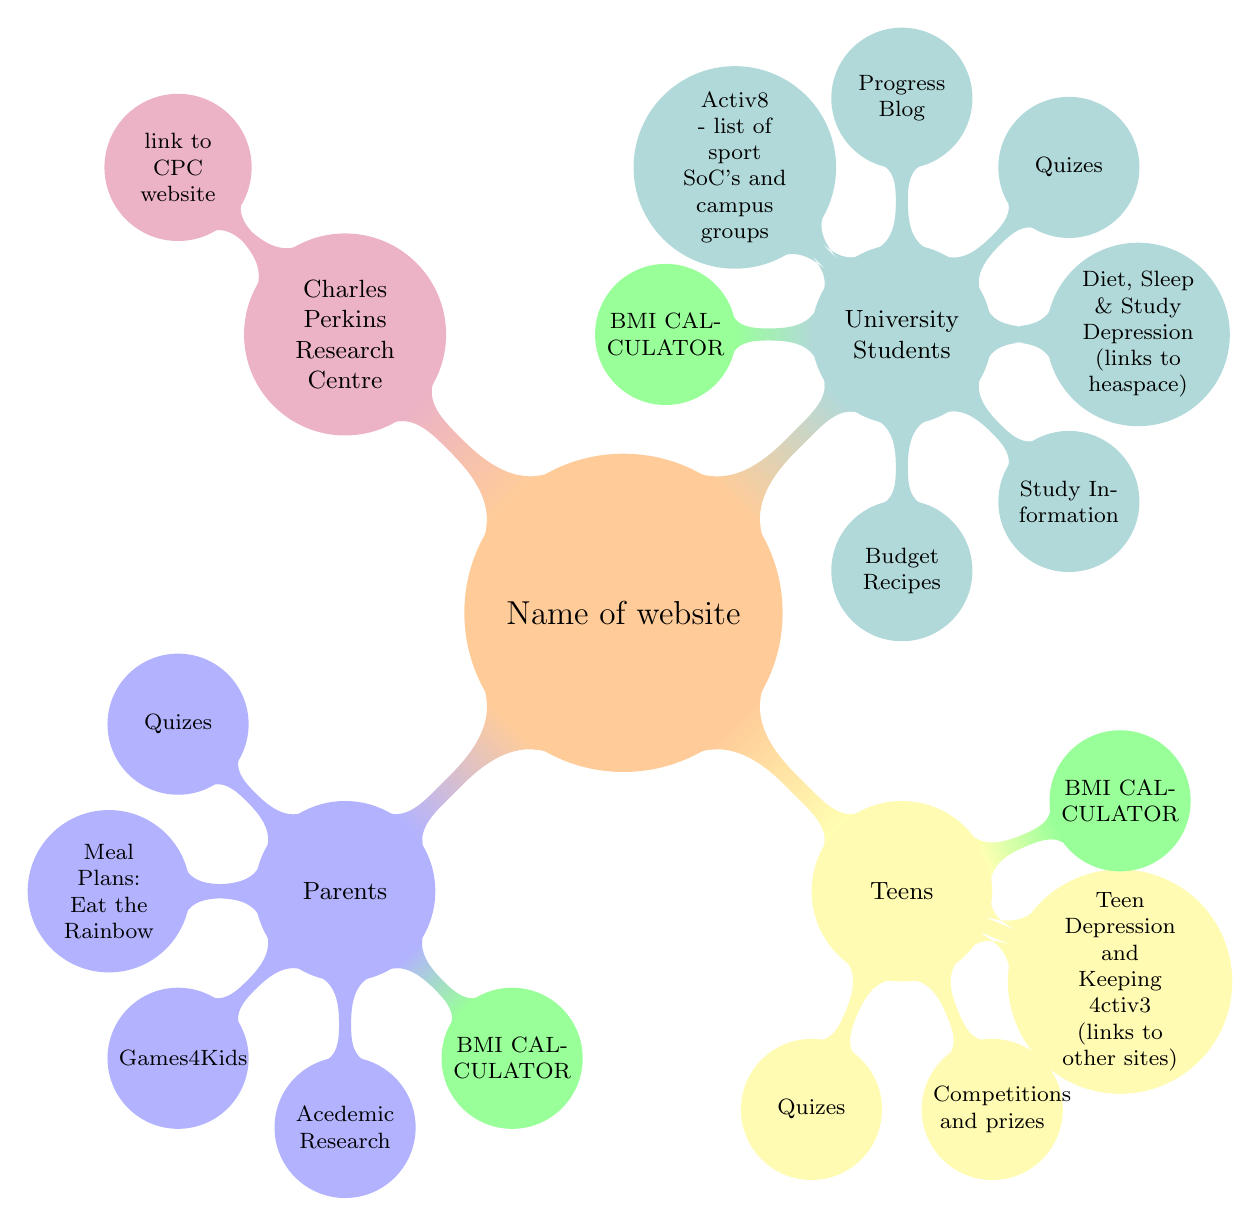
\begin{tikzpicture}[mindmap, grow cyclic, every node/.style=concept,
      concept color=orange!40,
      level 1/.append style={level distance=5cm,sibling angle=90},
      level 2/.append style={level distance=3cm,sibling angle=45},]
  %.
  \node{Name of website}
     child [concept color=blue!30] { node {Parents}
          child { node {Quizes}}
          child { node {Meal Plans: Eat the Rainbow}}
          child { node {Games4Kids}}
          child { node {Acedemic Research}}
          child [concept color=green!40] { node {BMI CALCULATOR}}
      }
      child [concept color=yellow!30] { node {Teens}
          child { node {Quizes}}
          child { node {Competitions and prizes}}
          child { node {Teen Depression and Keeping 4ctiv3 (links to other sites)}}
          child [concept color=green!40] { node {BMI CALCULATOR}}
      }
      child [concept color=teal!30] { node {University Students}
          child { node {Budget Recipes}}
          child { node {Study Information}}
          child { node {Diet, Sleep \& Study Depression (links to heaspace)}}
          child { node {Quizes}}
          child { node {Progress Blog}}
          child { node {Activ8 - list of sport SoC's and campus groups}}
          child [concept color=green!40] { node {BMI CALCULATOR}}
      }
      child [concept color=purple!30] { node {Charles Perkins Research Centre}
          child { node {link to CPC website}}
      };
  %.
  \end{tikzpicture}
  \caption{Sub-domain Hierarchy}
  \label{fig:subdomain-hierarchy}
\end{figure}

.
% include site_map.txt
%
% Copyright © 2014 Sara Lelliott. All Rights Reserved.
%
\begin{verbbox}

                                            +--------+ +------+   +--------+
                                            |register| |log in|   |site map|
                                            +--------+ +------+   +--------+



                                +-------------+
                                |contact us/  |
                                | credits     |
  +--------------------+        +---+---------+
  |                    |            |
  | home               +------------+--------------+
  |                    | +----------+-----+   +----+-----------+
  |                    | |about us/mission|   |CHARLES PERKINS |
  +-+-+------------+---+ | statement      |   | SITE           |
    | |            |     +-----+----------+   +----------------+
    | |            |
    | |            |
    | |   +--------v------+       +---------------+     +--------------+
    | |   |parents        +-------> BMI           +-----+ kids         |
    | |   +-----+---------+       +----+----------+     +----+---------+
    | |         |                      |                     |
    | |         |                      |                     |
    | |   +-----v--------+             |                     |
    | |   |meal plans    |       +-----v---------+    +------v-----------+
    | |   +-----+--------+       |quiz           |    | games            |
    | |         |                +---------------+    +------------------+
    | |   +-----+--------+
    | |   |blog          |
    | |   +--------------+
    | |
    | |
    | |
    | |
    | |
    | |  +--------------+      +----------+
    | +--+ teens        +------+ quizes   |
    |    +--------+-----+      +----------+
    |             |
    |             |           +--------------+
    |             +-----------+ BMI          |
    |                         | CALCULATOR   |
    |                         +--------------+
    |
    |
    |    +--------------+      +----------+
    +----+ uni students +------+ blog     |
         +---+----------+      +----------+
             |
             |           +--------------+
             +-----------+ BMI          |
                         | CALCULATOR   |
                         +--------------+

\end{verbbox}
\resizebox{0.95\textwidth}{!}{\theverbbox}


\section{End User Types}
\subsection{Parents and Kids}

This page will consist of information on what childhood obesity is and contain statistics on how many Australian children are affected by this disease and other associated health risks. There will be a link to a BMI calculator, quizzes that parents can do with their child, an interactive game called "Eat the Rainbow" which encourages healthy food choices and pictures of physical activities that can be fun to encourage kids to play outside and develop positive habits to help them in later years. There will also be Information on developing healthy meal plans and recipes that cater to gluten free, dairy free, halal, kosher and vegan diets and a survey to ascertain qualitative data about the website.

%%%%%%%%%%%%%%%%
% End Document %
%%%%%%%%%%%%%%%%
\end{document}
%.
